\documentclass[a4paper,12pt]{article}
\usepackage[utf8]{inputenc}
\usepackage[T2A]{fontenc}
\usepackage[russian,english]{babel}
\usepackage[pdftex]{graphics}
\DeclareGraphicsExtensions{.pdf,.png,.jpg}
\graphicspath{{pictures/}}
\begin{document}
\begin{center}
Санкт-Петербургский государственный политехнический университет
\\Кафедра компьютерных систем и программных технологий
\end{center}
\vspace*{10em plus .6em minus .5em}

\begin{center}
{\LARGEТелекоммуникационные технологии
\\Лабораторная работа №6
\\Цифровая модуляция}
\end{center}

\vspace*{5em plus .6em minus .5em}
\begin{flushright}
Выполнил:\\студент гр.33501/4\\Курякин Д. А.\\Проверила:\\Богач Н.В.
\end{flushright}

\vspace*{15em plus .6em minus .5em}
\begin{center}
{\smallСанкт-Петербург
\\2018}
\end{center}
\pagestyle{empty}
\newpage
\pagestyle{plain}

\section{Цель}

Изучение методов модуляции цифровых сигналов.

\section{Постановка задачи}

\begin{itemize}
\item Получить сигналы BPSK, PSK, OQPSK, genQAM, MSK, MFSK
модуляторов
\item Построить их сигнальные созвездия
\item Провести сравнение изученных методов модуляции цифровых
сигналов
\end{itemize}

\section{Теоретическое обоснование}

Фазовая манипуляция является широко используемым способом цифровой модуляции, при которой данные кодируются путем изменения фазы несущего сигнала. Сигнал на несущей частоте с фазой 0 декодируется как один бит или набор битов, а с фазой 90 - как другой бит. Имеется два основных метода декодирования таких сигналов:
\begin{itemize}
 \item Дифференциальный 
 \item Недифференциальный
\end{itemize}

Демодулятор, содержащий специальную схему PSK модуляции, может сравнивать фазу входящего сигнала с опорным сигналом или же сравнивать только изменения в фазе сигнала на несущей частоте, как это происходит при определении следующего символа.

PSK – это метод, при котором фаза несущего сигнала соответствует определенному символу. При недифференциальном кодировании на демодулятор подается опорный сигнал, который сравнивается с входящим сигналом. Разность фаз, которая сопоставляется одному символу, впоследствии, если фаза принимаемого сигнала сдвигается на какую-то величину от фазы опорного сигнала, сопоставляется другому символу или набору символов. Таким образом, фазу предыдущего символа знать необязательно. Это облегчает декодирование, так как ненужным становится механизм запоминания. Недостатком метода является необходимость включения демодулятора с опорным сигналом для выполнения сравнения. PSK широко применяется в различных технологиях, включая ZigBee, WiFi и радиочастотную идентификацию. Некоторые из приложений рассматриваются ниже.

OQPSK – так обозначают манипуляцию, при которой квадратурный компонент сигнала задерживается на половину цикла. В результате компонент в фазе (I) и квадратурный компонент (Q) никогда не изменяются одновременно. Наибольшее преимущество этого факта проявляется в процессе усиления, поскольку уровень входящего сигнала практически не изменяется в промежутках между последовательными символами. Линейные усилители остаются линейными в ограниченном диапазоне амплитуд входного сигнала, и, если можно уменьшить амплитуду, будет проще подобрать соответствующий усилитель для конкретного приложения. Кроме того, такой усилитель потребует меньше мощности, что делает его идеально подходящим для ситуаций, где используется малая мощность, как, например, в случаях с ZigBee и радиочастотной идентификацией. Лучше всего это видно при сравнении фазовых траекторий QPSK без сдвига и со сдвигом.

Множество современных коммуникационных протоколов используют квадратурную
амплитудную модуляцию или QAM. Среди них, например, 802.11b беспроводной Ethernet (Wi-Fi) и цифровое видео-вещание (Digital Video Broadcast (DVB)), в которых применяется модуляция 64-QAM, а также новые беспроводные технологии, такие как WiMAX, 802.11n и HSDPA/HSUPA (новый стандарт передачи данных в сотовой связи). Таким образом, благодаря широкому использованию QAM, понимание этого способа модуляции необходимо.QAM модуляция предназначена для передачи цифровой информации путём периодического изменения фазы и амплитуды синусоидальной электромагнитной волны. Каждая комбинация фазы и амплитуды называется символом и кодирует цифровой поток битов.


\newpage

\section{Ход работы}

\begin{enumerate}

{\item Сигнальное созвездие BPSK
	\center{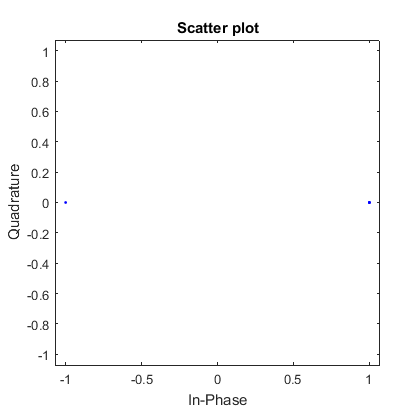
\includegraphics{./pictures/1.png}} \\ Рис.1 Сигнальное созвездие BPSK
	
	\center{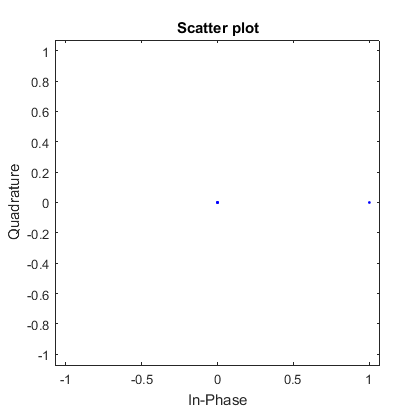
\includegraphics{./pictures/2.png} \\ Рис.2 Сигнальное созвездие BPSK}
	\\}

{\item Сигнальное созвездие PSK
	\center{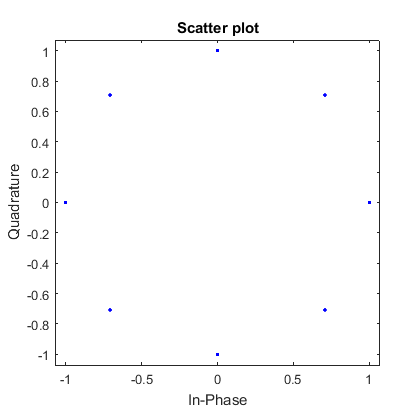
\includegraphics{./pictures/3.png} \\ Рис.3 Сигнальное созвездие PSK}
	
	\center{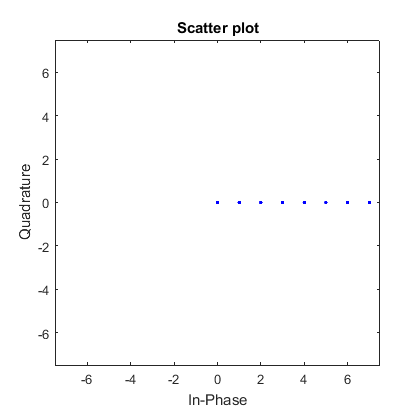
\includegraphics{./pictures/4.png} \\ Рис.4 Сигнальное созвездие PSK}
	\\}

{\item Сигнальное созвездие OQPSK
	\center{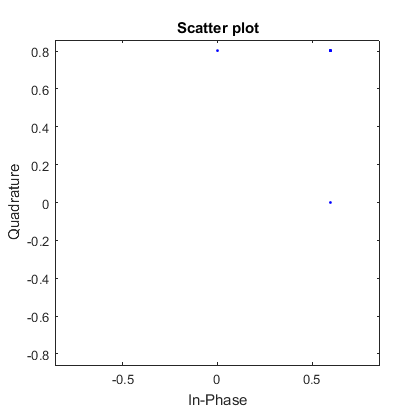
\includegraphics{./pictures/5.png} \\ Рис.5 Сигнальное созвездие OQPSK}
	
	\center{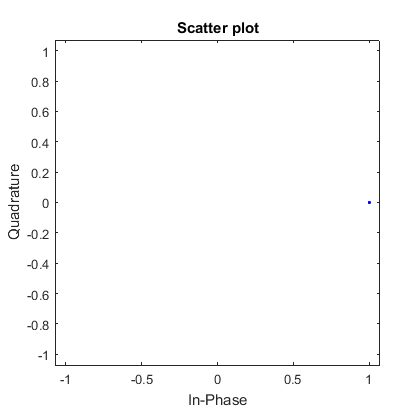
\includegraphics{./pictures/6.png} \\ Рис.6 Сигнальное созвездие OQPSK}
	\\}

{\item Сигнальное созвездие genQAM 
	\center{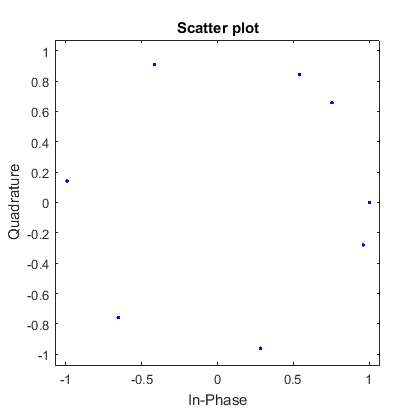
\includegraphics{./pictures/7.png} \\ Рис.7 Сигнальное созвездие genQAM}
	
	\center{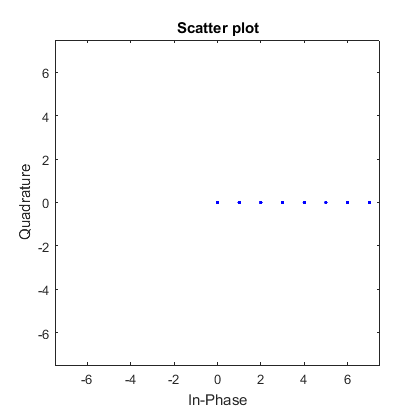
\includegraphics{./pictures/8.png} \\ Рис.8 Сигнальное созвездие genQAM}
	\\}

{\item Сигнальное созвездие MSK
	\center{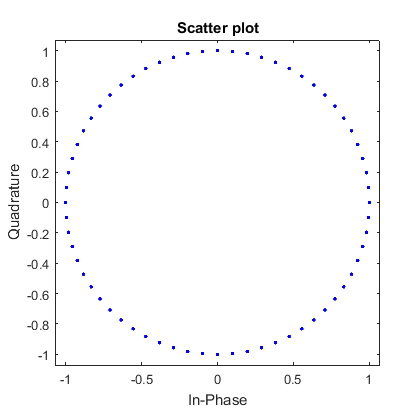
\includegraphics{./pictures/9.png} \\ Рис.9 Сигнальное созвездие MSK}
	
	\center{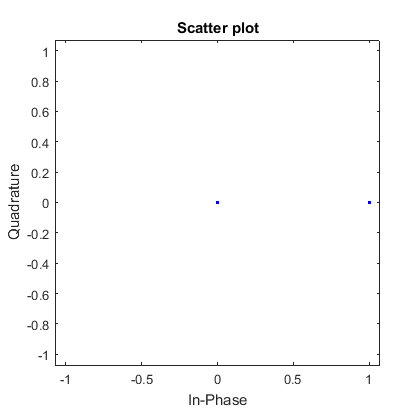
\includegraphics{./pictures/10.png} \\ Рис.10 Сигнальное созвездие MSK}
	\\}

{\item Сигнальное созвездие MFSK
	\center{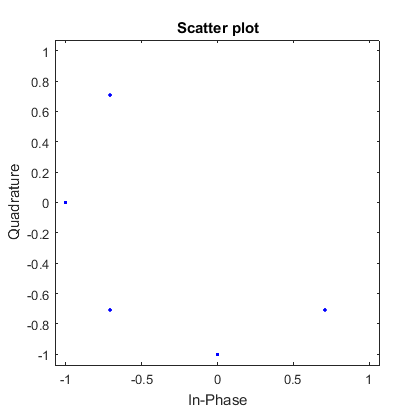
\includegraphics{./pictures/11.png} \\ Рис.11 Сигнальное созвездие MFSK}
	
	\center{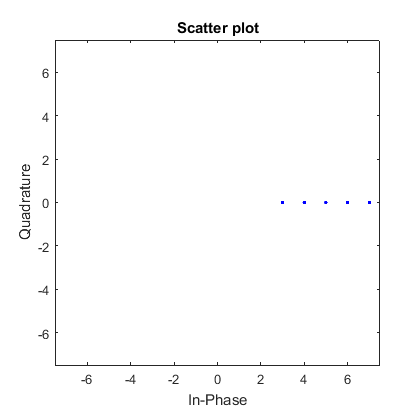
\includegraphics{./pictures/12.png} \\ Рис.12 Сигнальное созвездие MFSK}
	\\}

\end{enumerate}


\section{Вывод}

В технике цифровой связи методы модуляции играют весьма значительную роль. Помимо своей основной функции – преобразования символ – сигнал – процесс модуляции является составной частью общего процесса согласования сигнала с характеристиками канала.

Применение многопозиционной QAM способствует передаче большего количества информации, однако в реальных усло­виях, при наличии помех, на приемной стороне возможно ошибочное определение амплитуды и фазы передаваемого сигнала. Это обстоя­тельство и ограничивает количество информации, передаваемое од­ним символом. Тем не менее, основное преимущество QAM перед другими видами модуляции — в ее хорошей помехозащищенности. 

Способ модуляции PSK применяется в случаях, когда необхо­димо сохранить постоянной амплитуду передаваемого сигнала или исключить амплитуду из числа параметров, изменяемых в процессе модуляции. 

\end{document}
